\section{Artifical Neural Networks}
\label{sec:anns}

\acp{ANN} can generally be described as well-organised structures of mathematical computation and are inspired by the biological brain  \cite{ref:engelbrecht:2007}. \acp{ANN} have been successfully applied to a range of problem classes.  \citeauthor{ref:engelbrecht:2007}  \cite{ref:engelbrecht:2007} summarises some common problems that are solved using \acp{ANN}. These include classification  \cite{ref:khan:2001}, pattern matching  \cite{ref:cannady:1998, ref:kumar:1994}, pattern completion  \cite{ref:dayhoff:2001}, optimisation  \cite{ref:specht:1991} and data mining  \cite{ref:singh:2009}. \Acp{AN} provide the fundamental building blocks for \acp{ANN}.

\subsection{Artificial Neuron}
\label{sec:anns:an}

The \acs{AN} implements a non-linear mapping from some $I$-dimensional, real-numbered input space to some $T$-dimensional, real-numbered output space. The output space is usually in the ranges $[0,1]$ or $[-1,1]$, depending on the problem being solved \cite{ref:engelbrecht:2007}. The \acs{AN} implements various components and is illustrated in Figure  \ref{fig:artificial_neuron}.

\begin{figure}[htb]
	\centering
	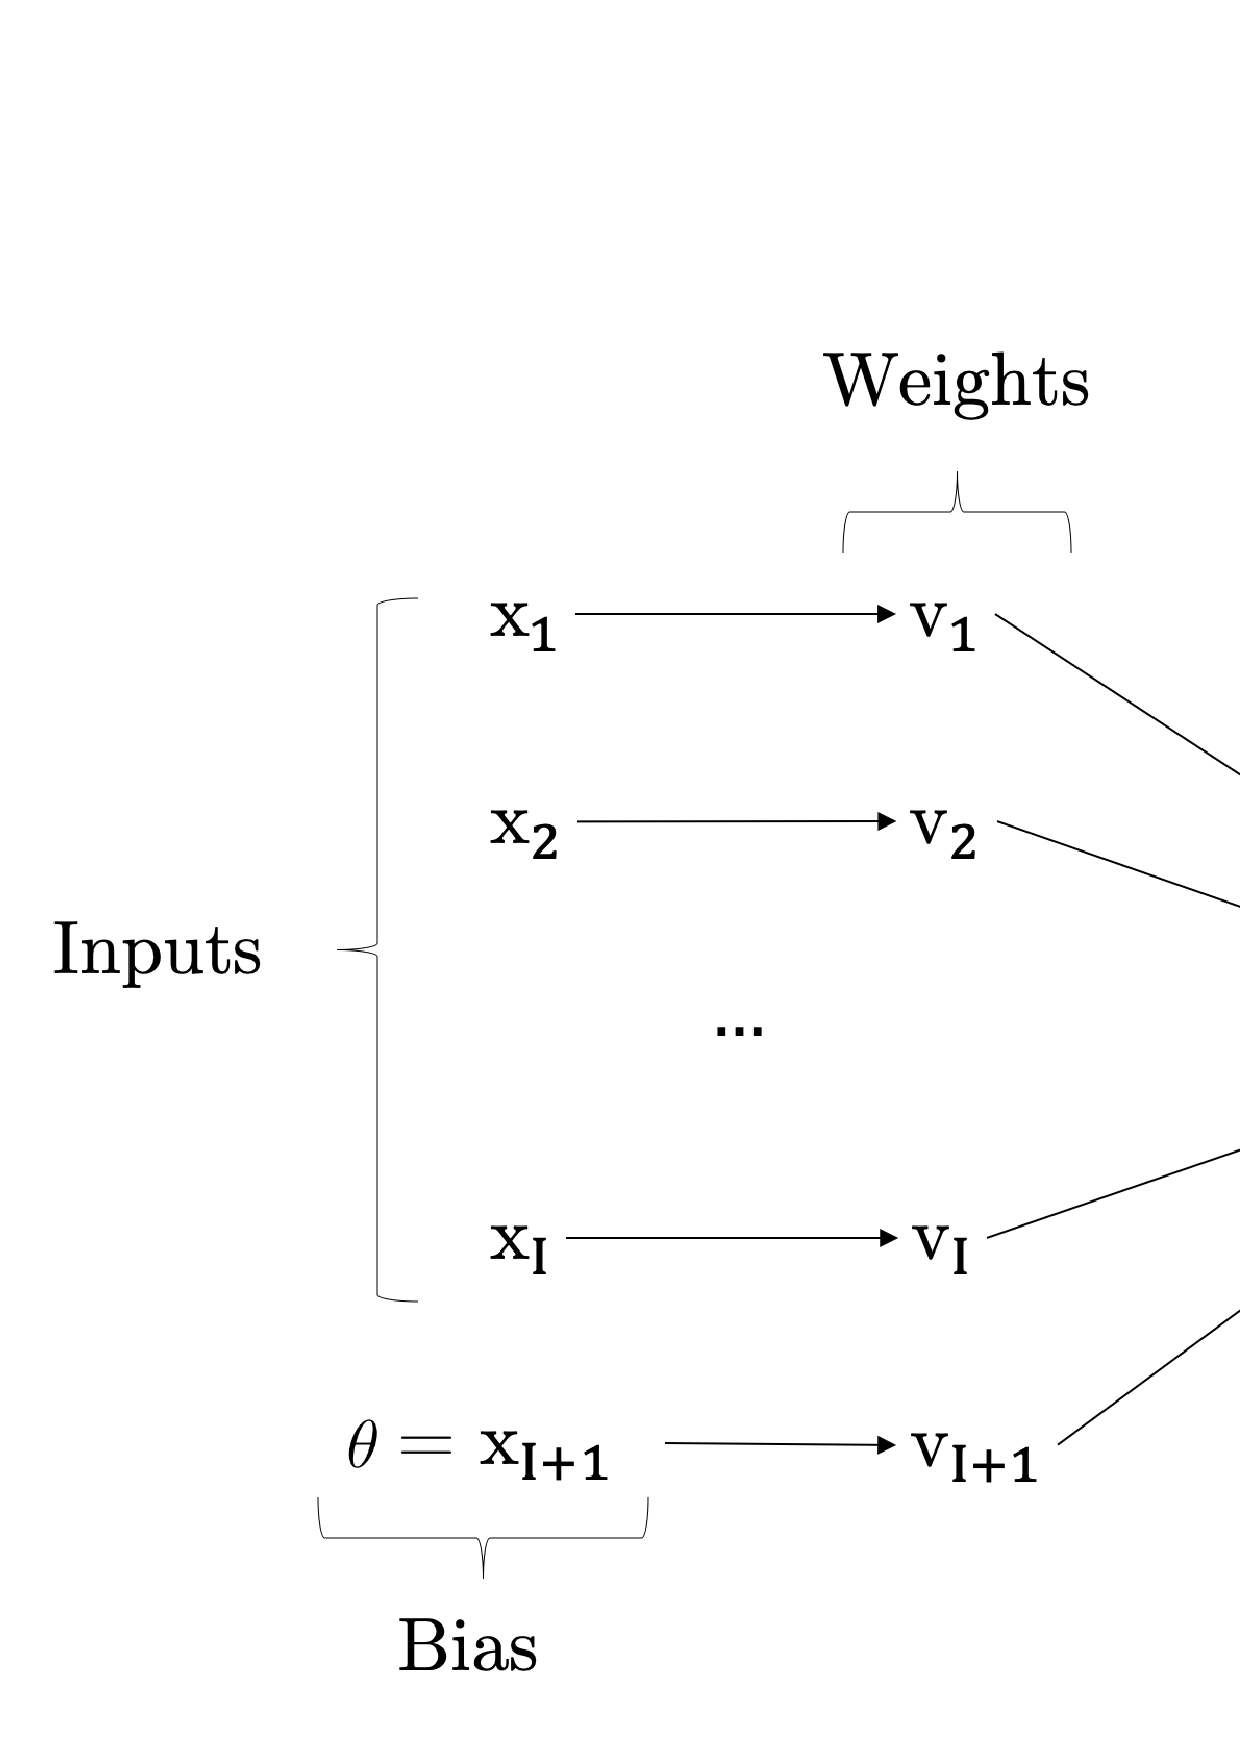
\includegraphics[width=\textwidth]{artificial_neuron.pdf}
	\caption[The \index{artificial neuron}artificial neuron]{An illustration of the \index{artificial neuron}artificial neuron.}
	\label{fig:artificial_neuron}
\end{figure}

Each of the components of the \acs{AN}, presented in Figure  \ref{fig:artificial_neuron}, is inspired by some element of the \acs{BN}. The input ($\boldsymbol{x}$) models the activations received from the pre-synaptic neuron. The weights ($\boldsymbol{v}$), model the \index{synapse}synapses and connection strengths. The \index{net input signal}net input signal ($net$) models the net resulting activations from all connected pre-synaptic neurons. The biases ($\theta$), model a mechanism introduced to influence the strength of the activation (output signal) of the \acs{AN}. The activation function ($f$) models the action potential of the \acs{BN} and is based on the net input signal. Finally, the output ($\boldsymbol{y}$) models the activation by the post-synaptic neuron.

\subsection{Feedforward Neural Networks}
\label{sec:anns:ffnn}

Multiple \acp{AN} can be organised and used together forming a ``network'' of \acp{AN} referred to as an \acf{ANN}. The architecture of the \acs{ANN} refers to the way in which \acp{AN} are organised. \acp{ANN} can be organised in layers where a single layer can contain multiple \acp{AN}. Generally, each layer makes use of the same \index{activation function}activation function. Output from one layer is propagated as input to the next layer. The topology of the \acs{ANN} refers to the way that layers of \acp{AN} are connected to each other. There are many different topologies  \cite{ref:miikkulainen:2010}.

This research focuses on a particular type of \acs{ANN}, referred to as \acp{FFNN}. \acp{FFNN} were the first and simplest type of \acp{ANN} developed  \cite{ref:schmidhuber:2015} and implement an architecture consisting of input, hidden and output layers by arranging them in sequential order. Furthermore, \acp{FFNN} implement \index{fully connected topology}fully connected topologies, where each \acs{AN} in one layer is connected to all \acp{AN} in the next, without any cycles  \cite{ref:zell:1994}.

In \acp{FFNN}, information moves forward, in one direction, from the input nodes, through the hidden nodes and finally to the output nodes. An illustration of a \acs{FFNN} is given in Figure  \ref{fig:ffnn}.

\begin{figure}[htb]
	\centering
	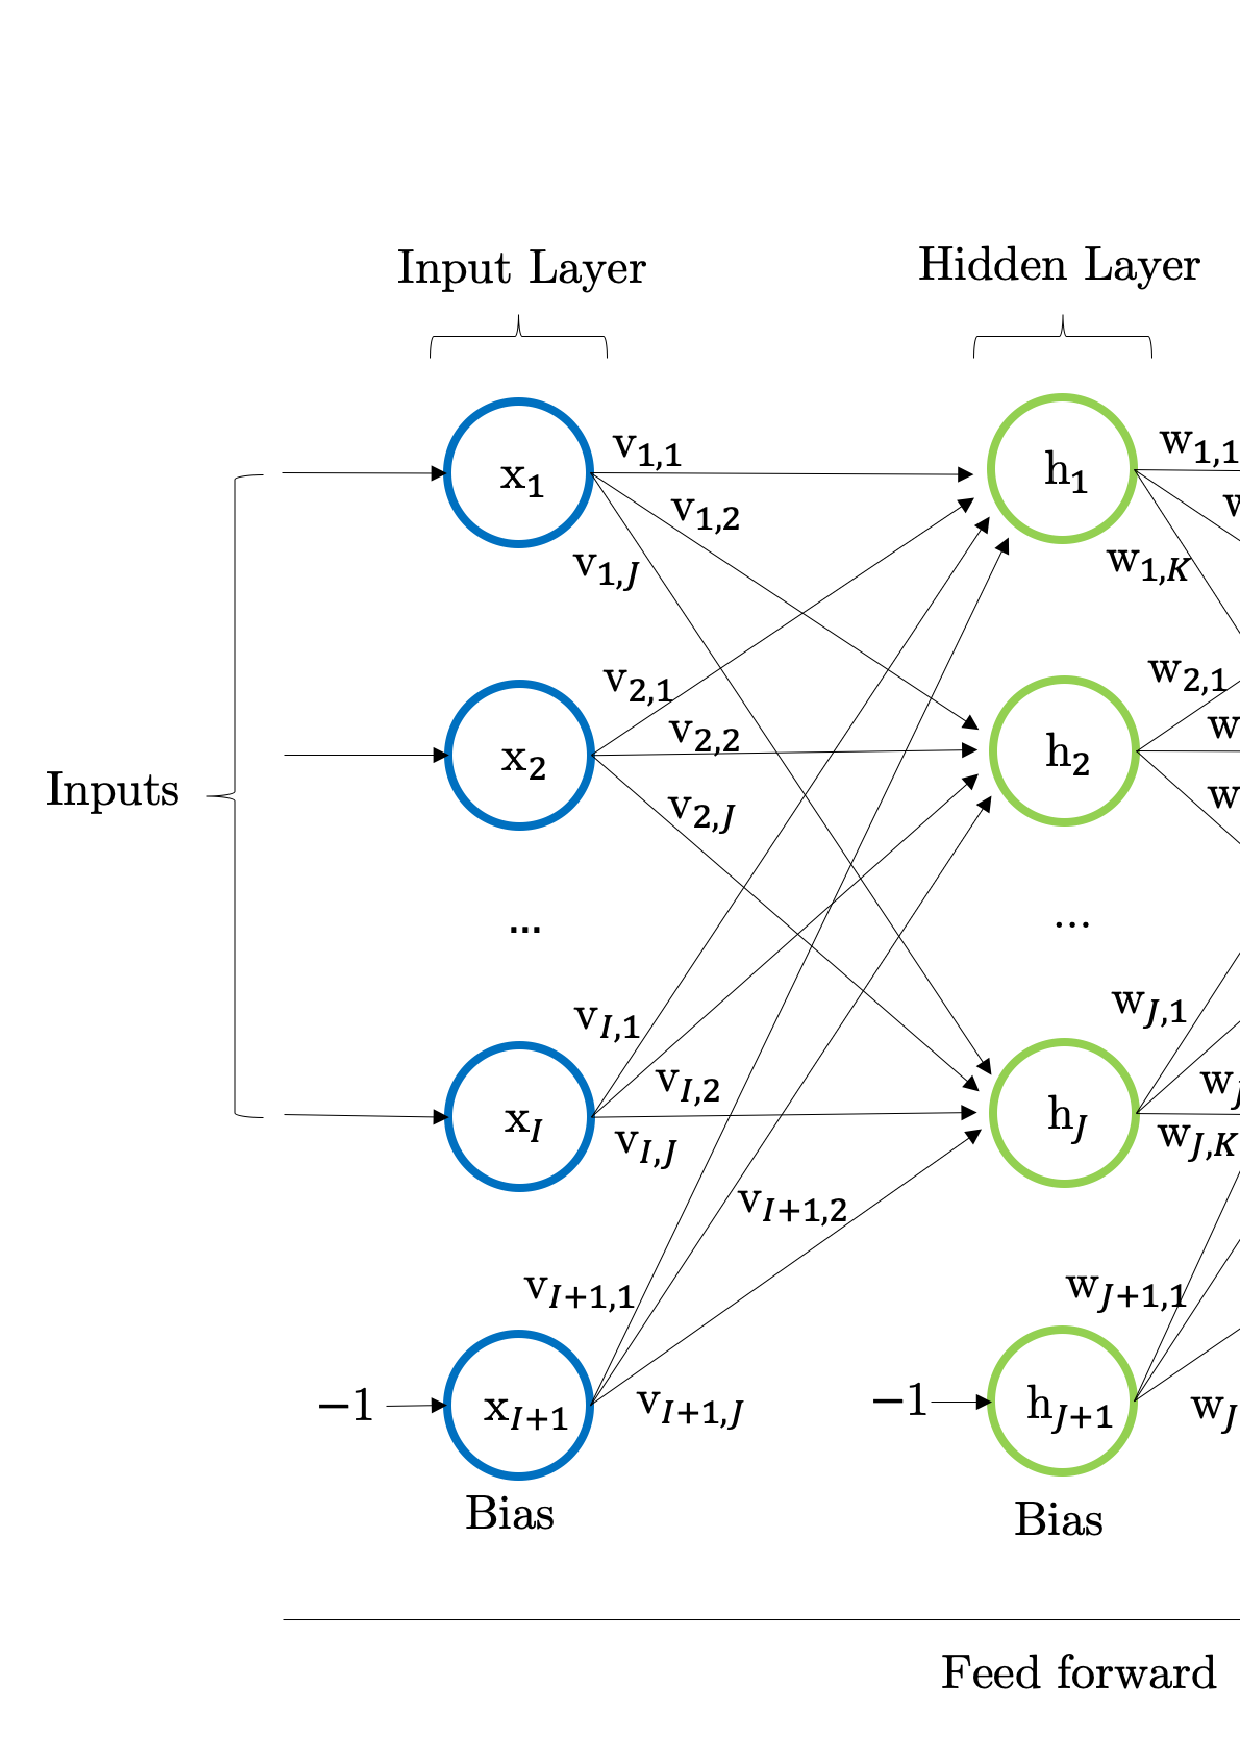
\includegraphics[width=0.98\textwidth]{feedforward_neural_network.pdf}
	\caption[A \index{feedforward neural network}feedforward neural network]{An illustration of a \index{feedforward neural network}feedforward neural network implementing input, hidden and output layers using a fully connected topology.}
	\label{fig:ffnn}
\end{figure}

In Figure  \ref{fig:ffnn}, $x_i$ refers to the $i$-th dimension in the input vector $\boldsymbol{x}$, $h_j$ refers to the $j$-th dimension in the hidden layer, $y_k$ refers to the $k$-th dimension in the output vector $\boldsymbol{y}$, $v_{i,j}$ refers to the weight associated with input node $x_i$ and the hidden node $h_j$, and $w_{j,k}$ refers to the weight associated with hidden node $h_j$ and the output node $y_k$.


\subsection{Training}
\label{sec:anns:training}

\textit{Training} is the process whereby the weights of the \acs{FFNN} are systematically changed with the aim of improving the \textit{performance} of the \acs{FFNN}. Finding the optimal weights that produce the best performance on a given task is an optimisation problem. The optimisation algorithm used to find the optimal weights is referred to as a \index{heuristic}\textit{heuristic}. \index{heuristic}Heuristics search for possible solutions in the solution-space and make use of information from the search space to guide to process.

During the training process, the \acs{FFNN} is exposed to data while trying to produce some target outcome. The degree to which the produced outcome differs from the target outcome is referred to as \textit{loss}. Since training of \acp{FFNN} is an optimisation problem, the goal of the training process is to minimise the loss. The loss is calculated using an error function. This research focuses on a number of error functions, including \acf{SSE}, \acf{MSE}, \acf{RMSE}, \acf{MAE}, \acf{BinXE}, \acf{CatXE} and \acf{SparseCatXE}.

\index{supervised learning}Supervised learning is the process of training where the data that is presented to the \acs{FFNN} during training, includes the desired solution  \cite{ref:geron:2017}. The \acs{FFNN} learns the mapping function from the input to the target output  \cite{ref:brownlee:2016}.
